\title{CS 613 - Machine Learning}
\author{
	Assignment 1 - Dimensionality Reduction \&  Clustering\\
	Alex Lapinski\\
	Fall 2016
}
\date{10/01/2016}
\documentclass[12pt]{article}
\usepackage[margin=0.7in]{geometry}
\usepackage{graphicx}
\usepackage{float}
\usepackage{comment}
\usepackage{amsmath}
\graphicspath{ {../graphs/raw/}{../graphics/clean/} }

\begin{document}
\maketitle
\section*{Part 1 - Answers to Theory Questions}
\begin{enumerate}
\item Why do we like to use quadratic error functions (say over a 4th degree polynomial function) (2pts)?

\noindent

The primary reason for using a quadratic error function is that there can only be one maximum or minum. 



\newpage
\item Consider the following data:\\
\begin{center}
$
 \begin{bmatrix}
	-2 & 1\\
	-5 & -4\\	
	-3 & 1\\
	0 & 3\\
	-8 & 11\\
	-2 & 5\\
	1 & 0\\
	5 & -1\\
	-1 & -3\\
	6 & 1\\
\end{bmatrix}
$
\end{center}
	\begin{enumerate}
	\item Find the principle components of the data (you must show the math, including how you compute the eigenvectors and eigenvalues).  Make sure you standardize the data first and that your principle components are normalized to be unit length (5pts).

\hfill \break
\hfill \break

$Mean_{col1} = \mu_1 = (-2 + -5 + -3 + 0 + -8 + -2 + 1 + 5 + -1 + 6)/10 = -0.9$\newline
$Mean_{col2} = \mu_2 = (1 + -4 + 1 + 3 + 11 + 5 + 0 + -1 + -3 + 1)/10 = 1.4$\newline
$Mean = \mu = \begin{bmatrix}-0.9 & 1.4\\ \end{bmatrix}$\newline
$Standard Deviation_{col1} = \sigma_1 = 4.22821213$\newline
$Standard Deviation_{col2} = \sigma_2 = 4.27395211$\newline
$Standard Deviation = \sigma = \begin{bmatrix} 4.22821213 & 4.27395211\\ \end{bmatrix}$\newline
\hfill \break
$Standardized Data = (Data - \mu) / \sigma =
\begin{bmatrix}
-0.260157 & -0.093590\\
-0.969677 & -1.263468\\
-0.496664 & -0.093590\\
 0.212856 & 0.374361\\
-1.679197 & 2.246165\\
-0.260157 & 0.842312\\
 0.449363 & -0.327566\\
 1.395389 & -0.561541\\
-0.023651 & -1.029492\\
 1.631895 & -0.093590\\
\end{bmatrix} 
$

TODO: Compute Covariance Matrix
$
\Sigma = \newline
\small
\begin{bmatrix}
0.0148723 & -0.02446792 & 0.03356939 &  0.01345069 & 0.32691793 & 0.0918175 & -0.06470532 & -0.16298003 & -0.08377002 & -0.14370452\\
-0.02446792 & 0.04315646 & -0.05920962 & -0.0237243 & -0.57661715 & -0.16194751 & 0.1141271 & 0.28746383 &  0.14775339 & 0.25346573\\
0.03356939 & -0.05920962 & 0.08123418 & 0.03254917 & 0.79110483 & 0.22218809 & -0.15657963 & -0.39439344 & -0.20271408 & -0.34774888\\
0.01345069 & -0.0237243 & 0.03254917 & 0.01304191 & 0.31698244 & 0.08902704 & -0.06273883 & -0.15802684 & -0.08122413 & -0.13933714\\
0.32691793 & -0.57661715 & 0.79110483 & 0.31698244 &  7.70423086 & 2.16379454 & -1.52486192 & -3.84082867 & -1.97414559 & -3.38657727\\
0.0918175 & -0.16194751 & 0.22218809 & 0.08902704 & 2.16379454 & 0.60771892 & -0.42826961 & -1.0787273 & -0.5544545 & -0.95114717\\
-0.06470532 & 0.1141271 & -0.15657963 & -0.06273883 & -1.52486192 & -0.42826961 &  0.3018087 & 0.76019703 & 0.39073329 & 0.6702892\\
-0.16298003 & 0.28746383 & -0.39439344 & -0.15802684 & -3.84082867 & -1.0787273 & 0.76019703 & 1.91478749 & 0.98418066 & 1.68832727\\
-0.08377002 & 0.14775339 & -0.20271408 & -0.08122413 & -1.97414559 & -0.5544545 & 0.39073329 & 0.98418066 & 0.50585852 & 0.86778248\\
-0.14370452 & 0.25346573 & -0.34774888 & -0.13933714 & -3.38657727 & -0.95114717 & 0.6702892 & 1.68832727 & 0.86778248 & 1.4886503\\
\end{bmatrix}
$
\normalsize

Now that we have the Covariance matrix, we plug it into the equation $\Sigma w = \alpha w$ and compute the eigen values and eigen vectors, where the eigen values will be $\alpha$ and the eigen vectors will be the vector $w$.\newline

We'll set the equation $|\Sigma - \alpha I|$ equal to zero, since real eigen values only exist if this is equal to zero.\newline

$|\Sigma - \alpha I| = 0$\newline


TODO: Compute EigenVectors and EigenValues of Covariance Matrix


\newpage
	\item Project the data onto the principal component corresponding to the largest eigenvalue found in the previous part (3pts).
	\end{enumerate}

\newpage
\item Consider the following data:\\
\begin{center}
Class 1 = 
$
 \begin{bmatrix}
	-2 & 1\\
	-5 & -4\\	
	-3 & 1\\
	0 & 3\\
	-8 & 11\\
	
\end{bmatrix}
$
, Class 2 = 
$
 \begin{bmatrix}
	-2 & 5\\
	1 & 0\\
	5 & -1\\
	-1 & -3\\
	6 & 1\\
\end{bmatrix}
$
\end{center}
	\begin{enumerate}
	\item Compute the information gain for each feature.  You could standardize the data overall, although it won't make a difference. (5pts).
\newpage
	\item Which feature is more discriminating based on results in part a (1pt)?
\newpage
	\item Using LDA, find the direction of projection (you must show the math).  Normalize this vector to be unit length.\\ \emph{Note: You don't not have to standardize the data since your computations should take into account the mean and standard deviations of the classes separately.}  (5pts).
\newpage
	\item Project the data onto the principal component found in the previous part (3pts).
\newpage
	\item Does the projection you performed in the previous part seem to provide good class separation?  Why or why not (1pt)?
	\end{enumerate}
\end{enumerate}

\newpage
\section*{Part 2 - PCA Result}
TODO: Include graph of visualization of the PCA Result
\section*{Part 3 - Visualization of k-means}
\subsection*{Initial Setup}
TODO: Insert Graph of initial setup visualization
\subsection*{Initial Cluster Assignment}
TODO: Insert graph of initial cluster assignment visualization
\subsection*{Final Cluster Assignment}
TODO: Insert graph of final cluster assignment visualization
\subsection*{Results}
TODO: Report how many iterations it took for the algorithm to terminate

\newpage
\section*{Raw Graphs}
\begin{figure}[H]
\begin{center}
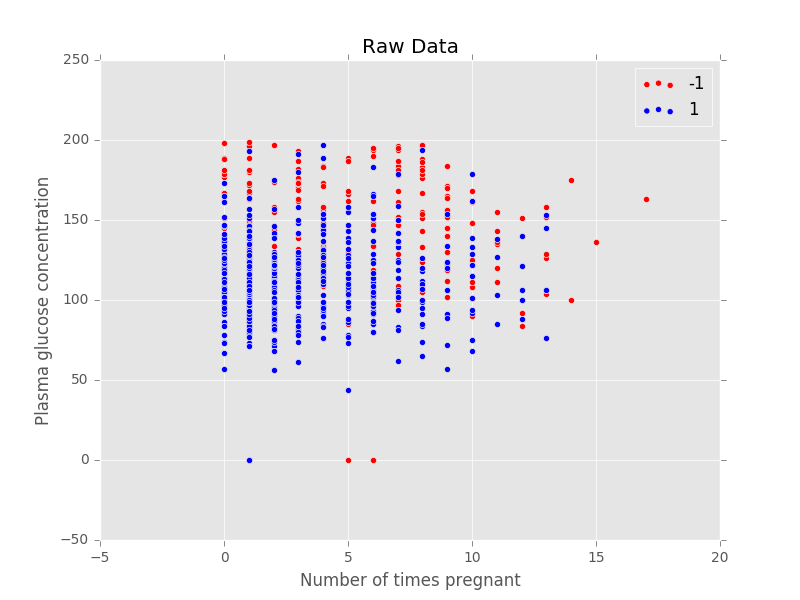
\includegraphics[scale=0.66]{graph1.png}
\caption{Raw Data 1}
\label{Raw Data 1}
\end{center}
\end{figure}

\begin{figure}[H]
\begin{center}
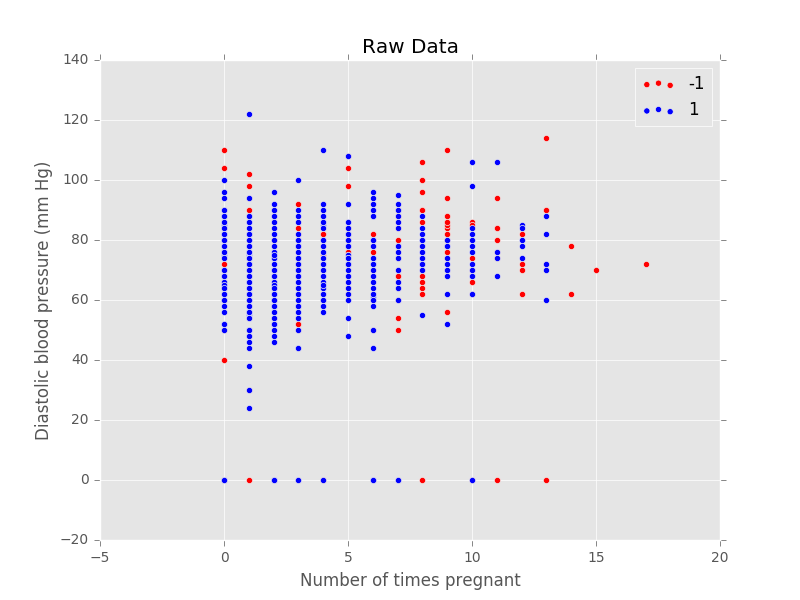
\includegraphics[scale=0.66]{graph2.png}
\caption{Raw Data 2}
\label{Raw Data 2}
\end{center}
\end{figure}

\begin{figure}[H]
\begin{center}
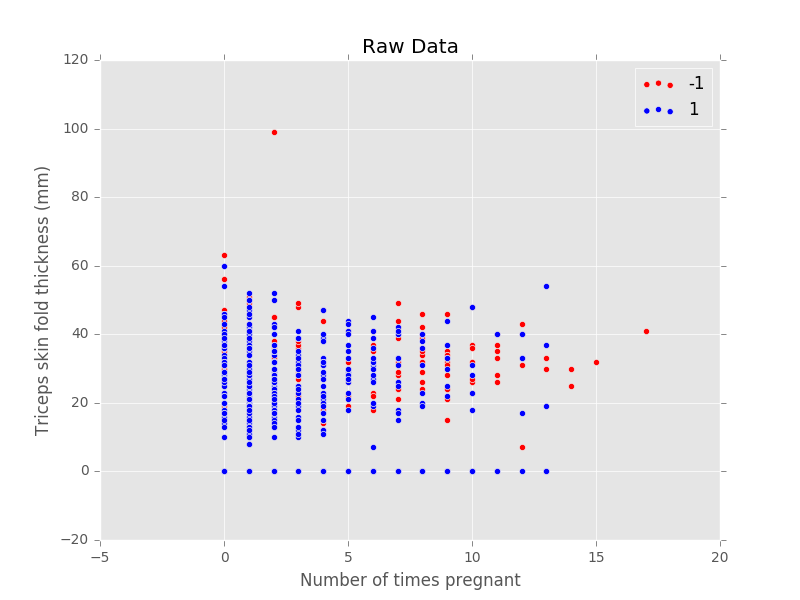
\includegraphics[scale=0.66]{graph3.png}
\caption{Raw Data 3}
\label{Raw Data 3}
\end{center}
\end{figure}

\end{document}

